\section{Introduction}

\subsection{Description de la societ\'e}
Australian Semiconductor Technology Company (ASTC) est un fournisseur mondial des solutions logicielles et matériels pour les systèmes embarqués. Cette soci\'et\'e propose des services de conception, validation et vérification des systèmes sur puces et les circuits intégrés. Elle a développé son outil VLAB, qui fournit des solutions innovantes, pour la simulation des logiciels embarqués sur les plateformes Hardware virtuelles. La société a son siège à Adélaïde en Australie, elle possède des bureaux et des centres de R\&D à Toulouse, Tokyo, Illinois, Austin, et Texas. 

ASTC Desing partners a été créée \`a toulouse par Nicolas Broueilh et Eric Faure en 2014. Cette partie est plus focalis\'e en la conception de logiciel embarqu\'e, sourtout la virtualisation de hardware avec VLAB Works. Le produit le plus develop\'e est la toolbox\footnote{Un toolbox de VLAB est un compilation des librairies qui ajoutent des modeles de simulation pour VLAB, par exemple, le toolbox Ethernet nous donne des noeuds Ethernet, ports et la class de trame Ethernet pour l'envoie d'information.} \textit{AURIX} qui est capable de virtualiser la famille \textit{aurix} de \textit{Infineon Technologies AG}. Dans la figure \ref{fig:vlab-presentation} on peut voir un exemple de vlab.

VLAB utilise python2 pour accéder a tous les éléments de hardware virtuel et évènements de la simulation comme les ports du microcontroleur, registres, connections virtuelles, temps de simulation, points d'arrête, entre autres. Pour les modèles de simulation il est utilis\'e $C++$ avec la librairie SystemC\cite{sysc}. Il y existe une API de SystemC pour python2 en raison de développer des mod\`eles plus rapidement mais moins performantes que celles en SystemC. %Toutes les mod\`eles doivent \^etre compil\'es avant de d\'emarrer la simulation.

%Para programar en vlab es necesario usar python2 y con este podemos acceder a todos los elementos de la simulacion. Para los modelos es necesario hacerlo usando C++ y SystemC. Hay una API de SystemC para python lo cual permite hacer pequenhos modelos mas rapido pero eso tendra un impacto en la velocidad de la simulacion si no son compilados. Para los modelos que necesitan mas performance es mejor usar SystemC.

%Aqui empiezo hablando de que es astc, que es una empresa internacional que hace herramientas de simulacion de microcontroladores. Explico un poco que es vlab, un par de capturas de pantalla con la que se muestre sus caracteristicas funcionales y zas, juera. 

%Finalmente digo que mi stage se trata de modelizar un gateway ya existente con la herramienta de simulacion.

\begin{figure}[!htb]
    \centering
        \subfigure[Vlab Logo]{
\includegraphics [width=2.5in]{img/VLAB_Works.png}}
        \subfigure[Vlab en marche]{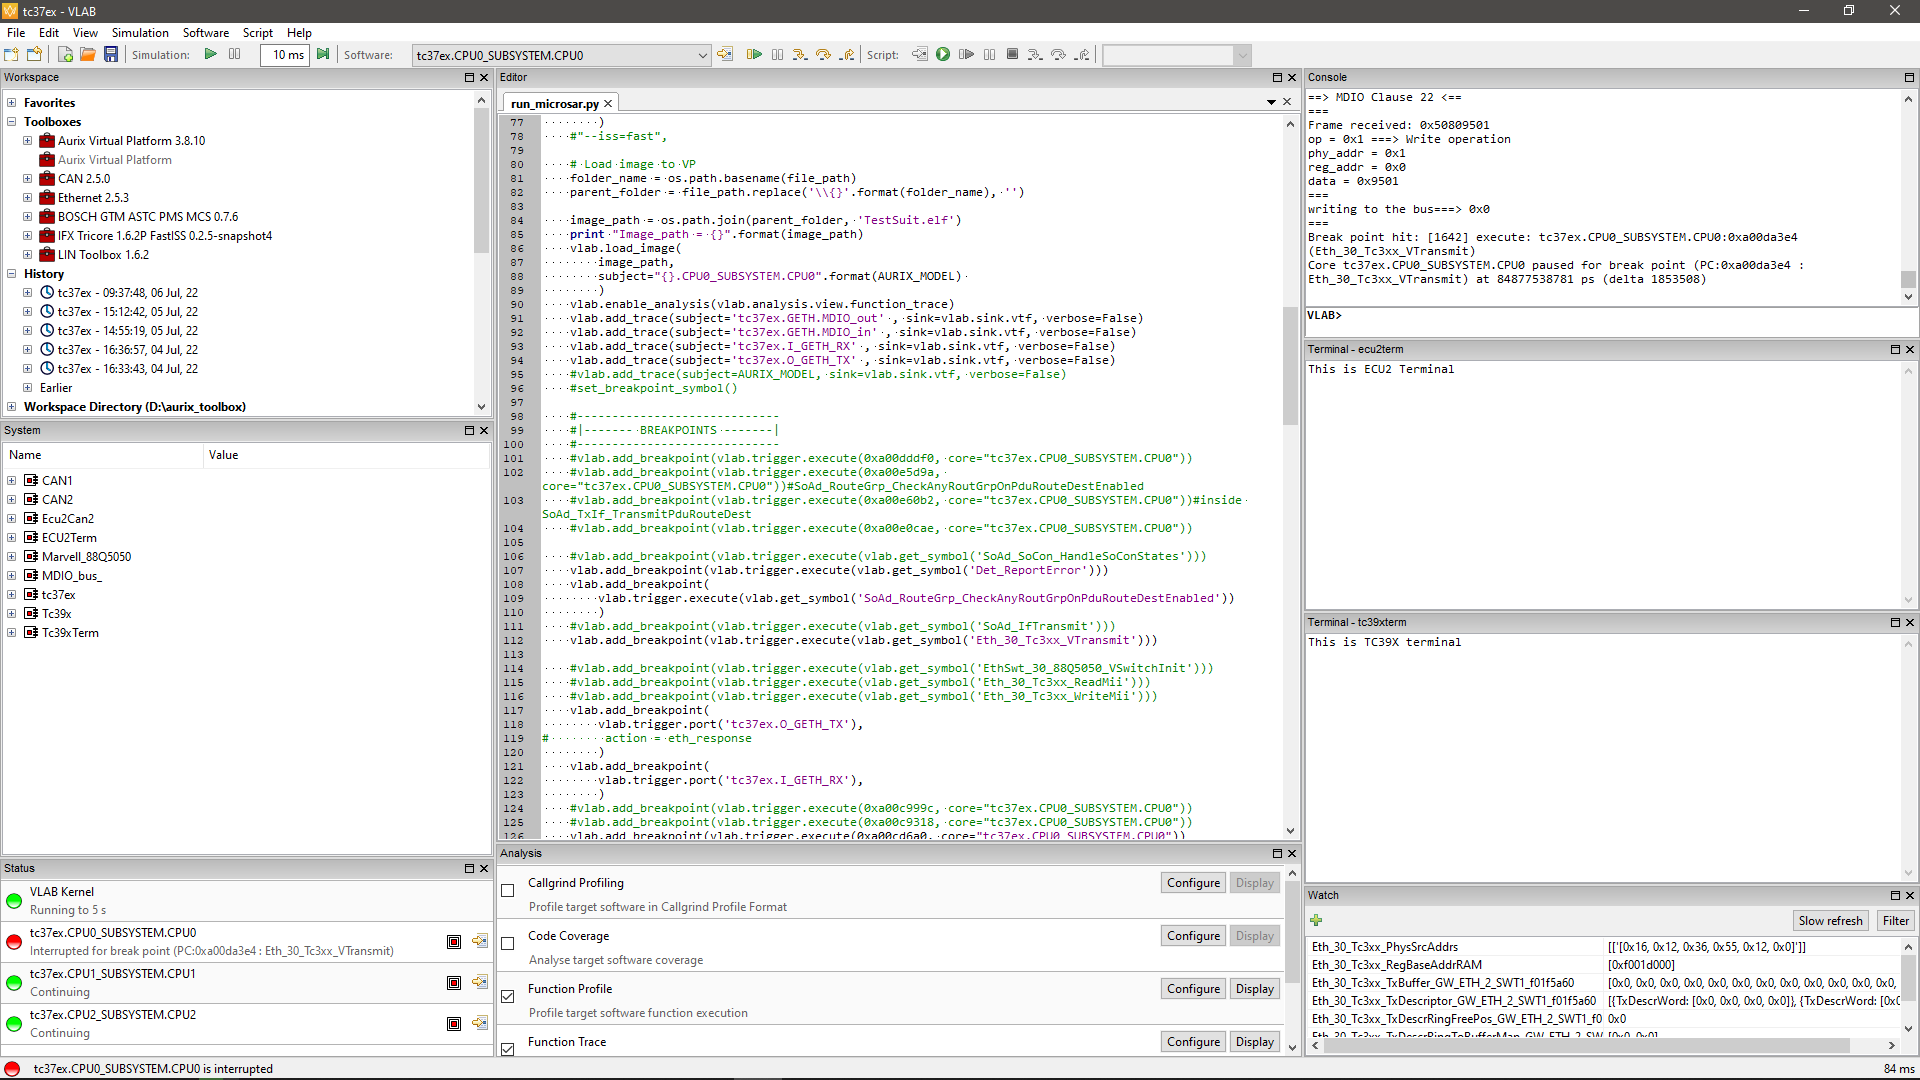
\includegraphics [width=5in]{img/vlab.png}}
    \caption{Vlab works}
    \label{fig:vlab-presentation}
\end{figure}

%\subsection{Virtualizacion y sus ventajas}
